\begin{center}
  \textbf{Exercices Théoriques - Analyse Numérique - 2017 \\
  Section MA \\
  Prof. A. Quarteroni \\
  Séance 3 - Systèmes linéaires : méthodes directes}
\end{center}


\vspace{10mm}

\begin{ex}
Considérons le cas particulier d'un système linéaire dont la matrice est tri-diagonale et inversible :

\begin{equation*}
  A = 
  \begin{bmatrix}
      a_1   & c_1     &             &   0        \\
      b_2   & a_2     & \ddots      &           \\
            & \ddots  & \ddots      & c_{n-1}        \\
        0   &         &    b_{n}    &     a_{n}
    \end{bmatrix}
    .
\end{equation*}

\begin{enumerate}[label=\alph*)]
  \item Montrer qu'il existe deux matrices bi-diagonales $L$ et $U$ de la forme
  
  \begin{equation*}
    L = 
    \begin{bmatrix}
          1       &         &             &   0        \\
        \beta_2   & 1       &             &           \\
                  & \ddots  &   \ddots    &          \\
          0       &         &  \beta_{n}  &     1
      \end{bmatrix}
      , 
      \quad
      U = 
      \begin{bmatrix}
            \alpha_{1}  &    \gamma_{1}     &             &   0        \\
                        &    \alpha_{2}     &    \ddots   &           \\
                        &                   &   \ddots    & \gamma_{n-1}     \\
            0           &                   &             & \alpha_{n}
        \end{bmatrix}
        ,
  \end{equation*}
  
  telles que $A = LU$, et donner les expressions des coefficients $\alpha_{i}$, $\beta_{i}$ et $\gamma_{i}$ en fonction des coefficients de $A$.
  Ces formules sont connues sous l'appellation d'\textit{Algorithme de Thomas}.
  
  \item Obtenir les formules résultantes de l'extension de l'algorithme de Thomas à la résolution du système $A \BoldX = \BoldF$, avec $\BoldF = \parent{f_{i}}^{n}_{i=1} \in \R^{n}$, donnée par
    \begin{enumerate}[label=(\alph*)]
      \item trouver $\BoldY$ tel que $L \BoldY = \BoldF$;
      \item trouver $\BoldX$ tel que $U \BoldX = \BoldY$.
    \end{enumerate}
    
  \item Combien d'opérations virgule flottante requiert l'algorithme précédent ?

\end{enumerate}









\end{ex}

\begin{sol}
\begin{enumerate}[label=\alph*)]
  \item On appelle $L_{i}$ la $i$-ième ligne de $L$ et $U_{j}$ la $j$-ième colonne de $U$.
        Il faut vérifier que
        
        \begin{equation*}
          L_{i} U_{j} = \squared{A}_{ij}.
        \end{equation*}
        
        Pour la matrice $A$, on a des éléments non nuls seulement pour $i = j$ ou $i = j \pm 1$.
        On obtient les équations suivantes :
        
        \begin{itemize}
          \item si $i = j$, on a $\beta_{i} \gamma_{i-1} + \alpha_{i} = a_{i}$;
          \item si $i = j - 1$, on a $\gamma_{i} = c_{i}$;
          \item si $i = j + 1$, on a $\beta_{i} \alpha_{j} = b_{i}$.
        \end{itemize}
        
        Donc, $\alpha_{i}$, $\beta_{i}$ et $\gamma_{i}$ s'obtiennent facilement avec les relations suivantes :
        
        \begin{equation}
        \label{eq:fact}
          \alpha_{1} = a_{1}, \quad 
          \beta_{i} = \dfrac{b_{i}}{\alpha_{i-1}}, \quad 
          \alpha_{i} = a_{i} - \beta_{i} c_{i-1}, \quad 
          \gamma_{i} = c_{i}.
        \end{equation}
        
  \item La résolution du système $A \BoldX = \BoldF$ revient à résoudre deux systèmes bidiagonaux, $L \BoldY = \BoldF$ et $U \BoldX = \BoldY$, pour lesquels on a les formules suivantes :
  
        \begin{equation}
        \label{eq:subst}
          \begin{split}
              \parent{L \BoldY = \BoldF} :  & \quad   y_{1} = f_{1}, \quad y_{i} = f_{i} - \beta_{i} y_{i-1}, \quad i = 2, \dots, n, \\
              \parent{U \BoldX = \BoldY} :  & \quad   x_{n} = \dfrac{y_{n}}{\alpha_{n}}, \quad x_{i} = \dfrac{y_{i} - \gamma_{i} x_{i+1}}{\alpha_{i}}, \quad i = n-1, \dots, 1.
          \end{split}
        \end{equation}
        
  \item L'algorithme requiert $8n - 7$ flops : $3 \parent{n-1}$ flops pour la factorisation \eqref{eq:fact} et $5n - 4$ flops pour la substitution \eqref{eq:subst}.
        
        
        
        
\end{enumerate}
\end{sol}

\begin{ex}
On considère un câble élastique qui occupe au repos le segment $\squared{0, 1}$, fixé aux extrémités, sur lequel on applique une force d'intensité $f \parent{x}$.
Son déplacement au point $x$, $u \parent{x}$, est la solution de l'équation différentielle suivante :

\begin{equation}
\label{eq:equadiff}  
  \begin{split}
      &  - u'' \parent{x} = f \parent{x}, \quad x \in \parent{0, 1}, \\
      &  u \parent{0} = 0, \quad u \parent{1} = 0.
  \end{split}
\end{equation}

Soit $N \in \N$, $h = 1/N$ et $x_{i} = ih$ pour $i = 0, \dots, N$; pour approcher la solution $u \parent{x}$, on considère la discrétisation de l'intervalle $\parent{0, 1}$ en $N$ sous-intervalles $\parent{x_{i}, x_{i+1}}$, et on construit une approximation $u_{i}$ de $u \parent{x_{i}}$ par la méthode des différences finies.
Cette méthode requiert de résoudre numériquement le système linéaire tridiagonal $A \BoldU = \BoldB$ qui suit :

\begin{equation}
\label{eq:systri}
  \dfrac{1}{h^{2}}
  \begin{bmatrix}
        2       &   -1    &             &         &     \\
       -1       &   2     &      -1     &         &     \\
                & \ddots  &   \ddots    &  \ddots &     \\
                &         &      -1     &     2   &  -1   \\
                &         &             &    -1   &   2
  \end{bmatrix}
  \begin{bmatrix}
    u_{1} \\
    u_{2} \\
    \vdots \\
    u_{N-2} \\
    u_{N-1} 
  \end{bmatrix}
  =
  \begin{bmatrix}
    f \parent{x_{1}} \\
    f \parent{x_{2}}  \\
    \vdots \\
    f \parent{x_{N-2}}  \\
    f \parent{x_{N-1}}  
  \end{bmatrix}
\end{equation}

où $\BoldU = \squared{u_{1}, u_{2}, \dots, u_{N-1}}^{\top}$ et $\BoldB = \squared{f \parent{x_{1}}, f \parent{x_{2}}, \dots, f \parent{x_{N-1}}}^{\top}$.
Plus $N$ est grand, plus l'approximation sera précise et plus la taille du système linéaire à résoudre sera élevée.

\begin{enumerate}[label=\alph*)]
  \item On suppose que la force appliquée soit $f \parent{x} = x \parent{1 - x}$ et on prend $N = 20$ intervalles.
        Construire la matrice $A$ et le vecteur $\BoldB$ correspondants, à l'aide des commandes suivantes :

\begin{verbatim}
f = @(x) x.*(1-x);
N = 20; h = 1/N;
x = linspace(h, 1-h, N-1)'; % on transpose pour avoir un vecteur colonne
b = f(x);
A = (N^2)*(diag(2*ones(N-1, 1),0) - diag(ones(N-2,1) - diag(ones(N-2,1),-1));
\end{verbatim}
        
        Calculer la factorisation $LU$ de $A$ avec la commande \textsc{MATLAB} \texttt{lu}.
        Vérifier que la matrice de permutation $P$ est l'identité (on sait de la théorie qu'aucune permutation de lignes n'est effectuée dès que la matrice est symétrique définie positive, ce qui est le cas de $A$).
        
        Calculer également la factorisation de Cholesky de $A$ (commande \texttt{chol}) et remarquer qu'elle diffère de la précédente.
        
        
  \item Mettre en oeuvre l'algorithme de \textit{substitution directe} pour la résolution d'un système triangulaire inférieure et l'algorithme de \textit{substitution rétrograde} pour la résolution d'un système triangulaire supérieure. Utiliser et compléter les fonctions suivantes :
  
        \lstinputlisting{s3/matlab/ex2_dir_incomplete.m}

        \lstinputlisting{s3/matlab/ex2_retro_incomplete.m}
  
        Calculer la solution du système linéaire $A \BoldU = \BoldB$ à partir de la factorisation $A = LU$, en utilisant les fonctions \texttt{subs\_directe} et \texttt{subs\_retrograde} pour résoudre les deux systèmes triangulaires.
  
  
  \item A l'aide de la commande \texttt{plot}, représenter le déplacement $\BoldU$ du câble aux noeuds $x_{i}$ définis au point 1.
  
  \item Etudier le comportement du conditionnement de la matrice $A$, $K \parent{A}$, lorsque $N$ augmente, en traçant le graphe des valeurs de $K \parent{A}$ pour $N = 10, 20, \dots, 120$.
        Tracer le graphe bilogarithmique des mêmes valeurs avec la commande \texttt{loglog}.
        Quel type de courbe obtient-on ?
        Si on suppose une relation linéaire $\log_{10} K \parent{A} = m \log_{10} N + c$ pour le graphe bilogarithmique, alors on a $K \parent{A} = C N^{m}$ (avec $C = 10^{c}$) : calculer les constantes $m$ et $C$.
        De combien $K \parent{A}$ croît-il lorsque on double le nombre $N$ des sous-intervalles ?
        
        
        
        
\end{enumerate}






\end{ex}

\begin{sol}
\begin{enumerate}[label=\alph*)]
  \item On définit la matrice $A$ et le vecteur $\BoldB$ avec les commandes suggérées dans l'énoncé :
  
\begin{verbatim}
  f = @(x) x.*(1-x);
  N = 20; h = 1/N;
  x = linspace(h, 1-h, N-1)'; 
  b = f(x);
  A = (N^2)*(diag(2*ones(N-1, 1),0) - diag(ones(N-2,1),1) - diag(ones(N-2,1),-1));
\end{verbatim}
        
        Ensuite, on calcule la factorisation $LU$ de $A$.
        En général, \textsc{MATLAB} peut décider d'effectuer des permutations de lignes pendant le processus de factorisation, ce qui mène à une factorisation $PA = LU$.
        Ainsi, la syntaxe de la commande \texttt{lu} à utiliser est la suivante :
        
\begin{verbatim}
  [L,U,P] = lu(A);
\end{verbatim}
        
        De cette façon, on a stocké dans la variable \texttt{P} la matrice de permutation $P$.
        Dans notre cas, on peut vérifier que \texttt{P} est la matrice identité : par exemple, on peut calculer l'écart maximal entre les éléments de $P$ et de $I$, et on obtient :
  
\begin{verbatim}
  max(max(abs(P - eye(N-1))))
  ans =
      0
\end{verbatim}
        
        Donc, \textsc{MATLAB} calcule la factorisation $LU$ sans permutation.
        Les facteurs ont été stockés dans les variables \texttt{L} et \texttt{U}.
        Ces facteurs diffèrent du facteur $H$ de la factorisation de Cholesky $A = H H^{\top}$, que l'on calcule avec la commande
  
\begin{verbatim}
  H = chol(A)';
\end{verbatim}
        
        car
        
\begin{verbatim}
  max(max(abs(L - H)))
  ans =
      27.2843
\end{verbatim}
        
  \item On trouve
  
        \lstinputlisting{s3/matlab/subs_directe.m}
        \lstinputlisting{s3/matlab/subs_retrograde.m}
        
        D'après le cours, on exploite la factorisation $LU$ de la façon suivante :
        
\begin{verbatim}
y = subs_directe(L,b);
u = subs_retrograde(U,y);
\end{verbatim}
        
  \item La Figure \ref{fig:solExacte} montre les déplacements $u_{i}$ aux noeuds $x_{i}$ (cercles rouges).
        Si $f \parent{x}$ est un polynôme, il est facile de trouver la solution exacte du problème différentiel : dans notre cas \footnote{Comme $u'' \parent{x} = - x + x^{2}$,
        on intègre deux fois et on trouve $u \parent{x} = x^{4} / 12 - x^{3} / 6 + a x + b$, où $a$ et $b$ sont deux constantes que l'on trouve en imposant les conditions aux bords :
          \begin{equation*}
            u \parent{0} = 0 \Longrightarrow b = 0, 
            \quad \quad
            u \parent{1} = 0 \Longrightarrow a = 1/12.
          \end{equation*}},
        on a $u \parent{x} = x^{4} / 12 - x^{3} / 6 + x / 12$.
        On a ajouté le graphe de $u \parent{x}$ afin de montrer qu'avec $N = 20$ sous-intervalles, on obtient déjà une solution approchée assez précise.
        La Figure \ref{fig:solExacte} a été obtenue par le script \texttt{ex2exact.m} suivant.
        
        \lstinputlisting{s3/matlab/ex2exact.m}
        
        
\begin{figure}[h!]
  \centering
  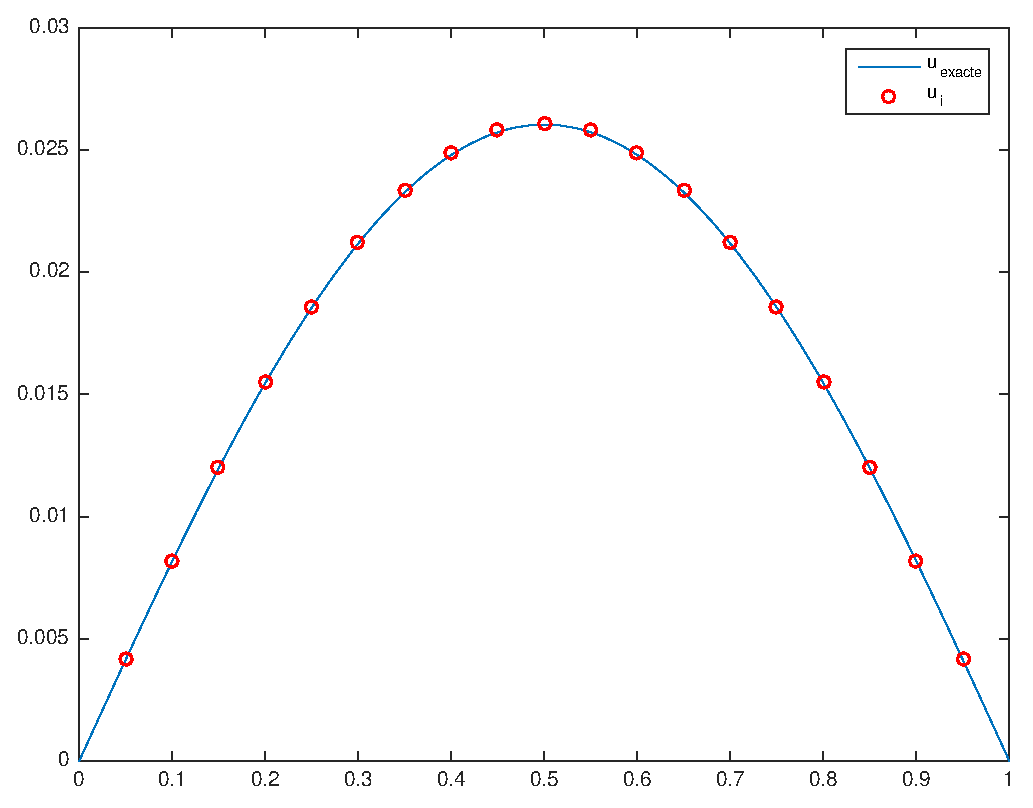
\includegraphics[scale = 0.5]{s3/matlab/ex2_uexact.eps}
  \caption{Solution exacte $u \parent{x}$ et déplacements approchés $u_{i}$}
  \label{fig:solExacte}
\end{figure}

        Il faut remarquer que la taille du vecteur $\BoldU$ est $N - 1$; en effet seules les valeurs des déplacements aux noeuds $x_{i}$ pour $i = 1, \dots, N - 1$ sont inconnues, car $u_{0} = u_{N} = 0$ (conditions aux bords).
        
  
  \item Pour chaque valeur de $N$, on a une matrice $A$ différente.
        Donc, il faut coder une boucle qui, pour $N = 10, 20, 30, \dots, 120$, construit cette matrice et calcule son conditionnement.
        Cette valeur sera ensuite mémorisée dans un vecteur \texttt{k}.
        La boucle peut se coder comme suit : 
        
\begin{verbatim}
for N = 10:10:120
  h = 1/N;
  A=(N^2)*(diag(2*ones(N-1,1),0)-diag(ones(N-2,1),1)-diag(ones(N-2,1),-1));
  k(N/10) = cond(A);
  disp(sprintf('N = %i: K(A) = %e',N,k(N/10)));
  % ceci pour afficher les valeurs calculees
end
\end{verbatim}        
        
        et on obtient
 
\begin{verbatim}
N = 10: K(A) = 3.986346e+01
N = 20: K(A) = 1.614476e+02

(...)

N = 110: K(A) = 4.903279e+03
N = 120: K(A) = 5.835434e+03
\end{verbatim} 

    Le graphe de $K \parent{A}$ en fonction de $N$ (commande \texttt{plot([10:10:120], k))} et le graphe bi-logarithmique (commande \texttt{loglog([10:10:120],k); grid on}) sont affichés en Figure \ref{fig:cond}.
    On peut trouver cette figure avec le script \texttt{ex2bilog.m}.
    
    \lstinputlisting{s3/matlab/ex2bilog.m}
    
    On voit que le graphe bi-logarithmique est bien celui d'une droite, donc du type
    
    \begin{equation*}
      \log_{10} K = m \log_{10} N + c.
    \end{equation*}
    
    On calcule $m$ et $c$ directement sur le graphe, en mesurant la pente entre les abscisses 1 $\parent{N = 10}$ et 2 $\parent{N = 100}$, ou bien en utilisant \MAT :
    
\begin{verbatim}
m = ( log10(k(10)) - log10(k(1)) ) / (log10(120) - log10(10))
m =
    2.0066
    
c = log10(k(1)) - m*log10(10)
c = 
    -0.4060
    
C = 10^c
C =
    0.3926
\end{verbatim} 

\begin{figure}[h!]
  \begin{subfigure}[b]{0.5\linewidth}
    \centering
    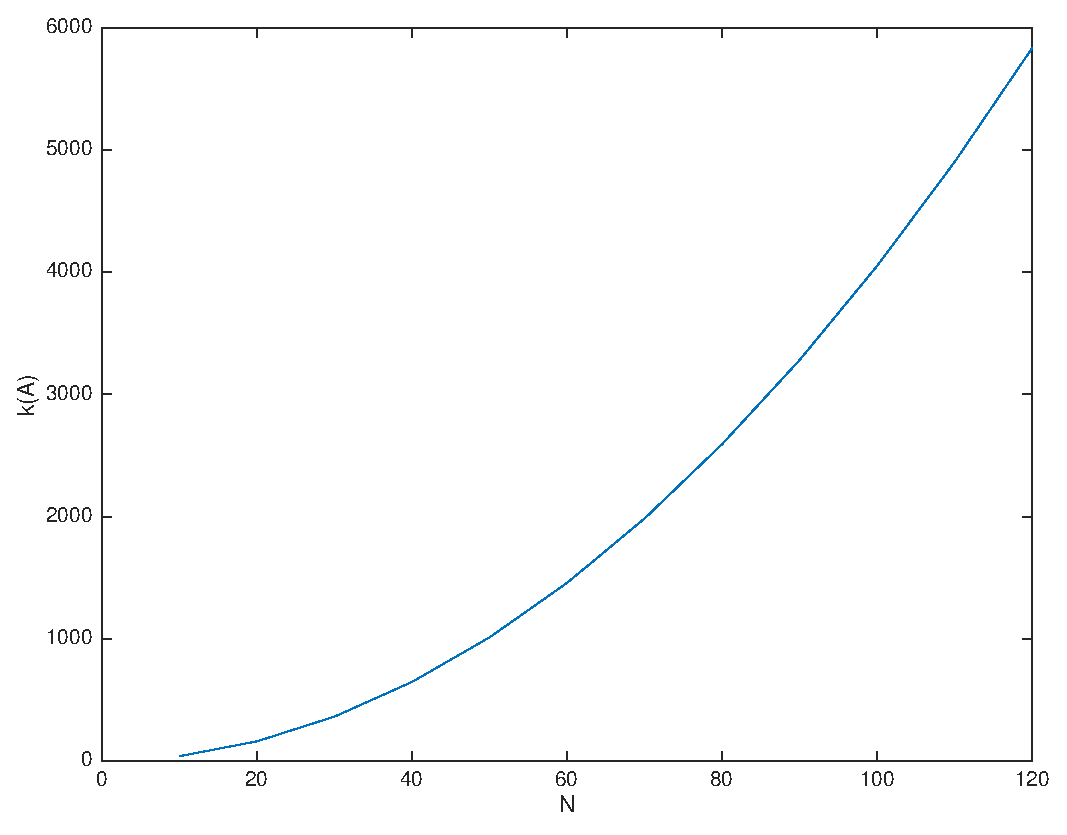
\includegraphics[scale=0.4]{s3/matlab/ex2_lin} 
    %\caption{Interpolation of $f$ using NCS \\ with $8+2$ points} 
    %\label{fig:q11_n8} 
  \end{subfigure}
  \begin{subfigure}[b]{0.5\linewidth}
    \centering
    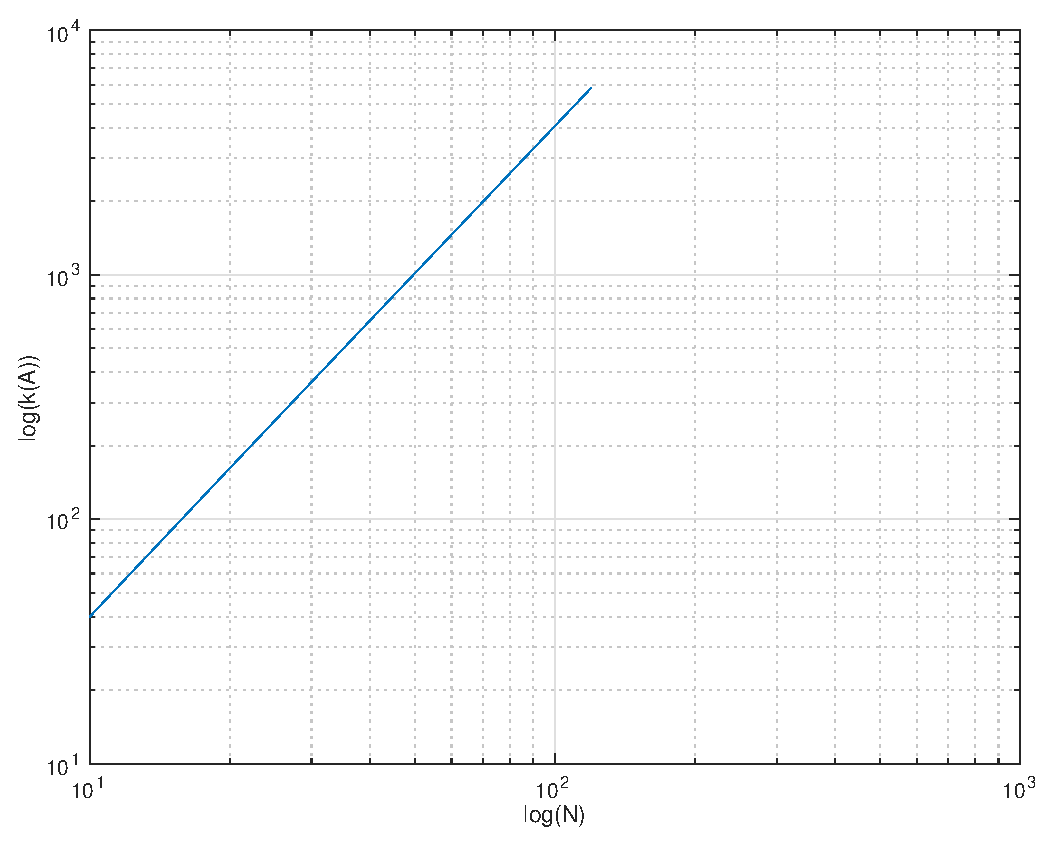
\includegraphics[scale=0.4]{s3/matlab/ex2_log} 
    %\caption{Interpolation of $f$ using NCS \\ with $8+2$ points} 
    %\label{fig:q11_n8} 
  \end{subfigure} 
  \caption{Nombre de conditionnement $K \parent{A}$ en fonction de $N$, graphes linéaire (à gauche) et bi-logarithmique (à droite)}
  \label{fig:cond}
\end{figure}

      La pente est presque égale à 2, donc la formule à proposer sera bien
      
      \begin{equation*}
        K \parent{A} = C N^{2}
      \end{equation*}
      
       avec $C \simeq 0.3926$.
       Donc, $K \parent{A}$ croît quadratiquement avec $N$, ce qui signifie que la solution du système linéaire par la méthode de factorisation $LU$ devient de plus en plus sensible aux perturbations sur les données et aux erreurs d'arrondi.

  


         
         
         
  
  
\end{enumerate}
\end{sol}

\begin{ex}
Etudier l'existence et l'unicité de la factorisation $LU$ des matrices suivantes :

\begin{equation*}
  A = \begin{bmatrix}
        1 & 2   \\
        1 & 2
      \end{bmatrix}
  , \quad
  B = \begin{bmatrix}
        0 & 1   \\
        1 & 0
      \end{bmatrix}
  , \quad
  C = \begin{bmatrix}
        0 & 1   \\
        0 & 2
      \end{bmatrix}
  .
\end{equation*}
\end{ex}

\begin{sol}
On rappelle que si $M \in \R^{n \times n}$, la factorisation $LU$ de $M$ avec $l_{ii} = 1$ pour $i = 1, \dots , n$ existe et est unique si et seulement si les sous-matrices principales $M_{i}$ de $M$ d'ordre $i = 1, \dots , n - 1$ sont inversibles (voir Théorème 3.4 à la page 77 du livre).
Dans ce cas :

\begin{equation*}
  M = \begin{bmatrix}
        1       & 0   \\
        l_{21}  & 1
      \end{bmatrix}
      \begin{bmatrix}
        u_{11} & u_{12}   \\
        0      & u_{22}
      \end{bmatrix}
  =
      \begin{bmatrix}
        u_{11}          & u_{12}   \\
        l_{21} u_{11}   & l_{21} u_{12} + u_{22}
      \end{bmatrix}
  .
\end{equation*}

La matrice singulière $A$, dont la sous-matrice principale $A_{1} = 1$ est inversible, admet une unique factorisation $LU$.
La matrice inversible $B$ dont la sous-matrice $B_{1}$ est singulière n'admet pas de factorisation,
tandis que la matrice (singulière) $C$, dont la sous-matrice $C_{1}$ est singulière, admet une infinité de factorisations de la forme $C = L_{\beta} U_{\beta}$,
avec $l^{\beta}_{11} = 1$, $l^{\beta}_{21} = \beta$, $l^{\beta}_{22} = 1$, et $u^{\beta}_{11} = 0$, $u^{\beta}_{12} = 1$, $u^{\beta}_{22} = 2 - \beta, \ \quad \forall \beta \in \R$.


\end{sol}

\begin{ex}
Soit $A$ la matrice donnée par

\begin{equation*}
  A = \begin{bmatrix}
        1  & 2  & 3  & 4  \\
        2  & 5  & 1  & 10  \\
        3  & 1  & 35 & 5  \\
        4  & 10 & 5  & 45 
      \end{bmatrix}
      ,
\end{equation*}

avec $\det \parent{A} > 0$.
Effectuer la factorisation de Cholesky de la matrice $A$, après avoir remarqué qu'une telle factorisation existe.

\end{ex}

\begin{sol}
La matrice est symétrique et définie positive.
En effet, la matrice est symétrique et tous les mineurs principaux dominants de $A$ sont positifs (critère de Sylvester).
On a vu au cours que les coefficients $h_{ij}$ de $H^{\top}$ (triangulaire inférieure), avec $A = H^{\top} H$, peuvent être calculés comme suit : $h_{11} = \sqrt{a_{11}}$ et, pour $i = 2, ... ,n$, on a

\begin{equation}
\label{eq:h}
  \begin{split}
      h_{ij}  = & \  \dfrac{1}{h_{jj}} \parent{a_{ij} - \sum_{k = 1}^{j-1} h_{ik} h_{jk}}, \quad j = 1, \dots, i-1; \\
      h_{ii}  = & \ \parent{a_{ii} - \sum_{k = 1}^{i-1} h_{ik}^{2}}^{1/2} .
  \end{split}
\end{equation}

On obtient ainsi

\begin{equation*}
  H^{\top} = \begin{bmatrix}
        1  & 0  & 0  & 0  \\
        2  & 1  & 0  & 0  \\
        3  & -5 & 1  & 0  \\
        4  & 2  & 3  & 4 
      \end{bmatrix}
      .
\end{equation*}

\end{sol}






